\documentclass[11pt]{article}

% For notes stored at notes/<domain>/<slug>/note.tex.
% Shared preamble for youtube_notes educational LaTeX notes.
% Intended for LuaLaTeX.

\usepackage[a4paper,margin=1in]{geometry}
\usepackage{fontspec}
\usepackage{microtype}
\usepackage{amsmath}
\usepackage{amssymb}
\usepackage{amsthm}
\usepackage{mathtools}
\usepackage{graphicx}
\usepackage{booktabs}
\usepackage{array}
\usepackage{xcolor}
\usepackage{enumitem}
\usepackage{tcolorbox}
\usepackage{tikz}
\usepackage{pgfplots}
\usepackage{siunitx}
\usepackage{hyperref}
\usepackage[nameinlink,noabbrev]{cleveref}

\pgfplotsset{compat=1.18}
\tcbuselibrary{breakable,skins}

\setmainfont{Latin Modern Roman}
\setsansfont{Latin Modern Sans}
\setmonofont{Latin Modern Mono}

\definecolor{ynBlue}{HTML}{1F4E79}
\definecolor{ynTeal}{HTML}{1B7F79}
\definecolor{ynGreen}{HTML}{2F7D32}
\definecolor{ynAmber}{HTML}{B86E00}
\definecolor{ynRed}{HTML}{A83232}
\definecolor{ynGray}{HTML}{F4F6F8}
\definecolor{ynInk}{HTML}{1F2933}

\hypersetup{
  colorlinks=true,
  linkcolor=ynBlue,
  citecolor=ynTeal,
  urlcolor=ynBlue,
  pdftitle={YouTube Note},
  pdfauthor={youtube_notes}
}

\setlist[itemize]{leftmargin=*,itemsep=0.2em,topsep=0.3em}
\setlist[enumerate]{leftmargin=*,itemsep=0.2em,topsep=0.3em}
\setlength{\parindent}{0pt}
\setlength{\parskip}{0.65em}

\numberwithin{equation}{section}

\theoremstyle{plain}
\newtheorem{theorem}{Theorem}[section]
\newtheorem{lemma}[theorem]{Lemma}
\newtheorem{proposition}[theorem]{Proposition}
\newtheorem{corollary}[theorem]{Corollary}

\theoremstyle{definition}
\newtheorem{definition}{Definition}[section]
\newtheorem{example}{Example}[section]

\theoremstyle{remark}
\newtheorem*{remark}{Remark}


% Common mathematical macros for generated notes.

\newcommand{\R}{\mathbb{R}}
\newcommand{\N}{\mathbb{N}}
\newcommand{\Z}{\mathbb{Z}}
\newcommand{\Q}{\mathbb{Q}}
\newcommand{\C}{\mathbb{C}}

\newcommand{\E}{\mathbb{E}}
\newcommand{\Var}{\operatorname{Var}}
\newcommand{\Cov}{\operatorname{Cov}}
\newcommand{\Corr}{\operatorname{Corr}}
\newcommand{\Prob}{\mathbb{P}}

\newcommand{\dd}{\,\mathrm{d}}
\newcommand{\grad}{\nabla}
\newcommand{\argmin}{\operatorname*{arg\,min}}
\newcommand{\argmax}{\operatorname*{arg\,max}}
\newcommand{\diag}{\operatorname{diag}}
\newcommand{\rank}{\operatorname{rank}}
\newcommand{\tr}{\operatorname{tr}}
\newcommand{\spanof}{\operatorname{span}}

\newcommand{\abs}[1]{\left\lvert #1 \right\rvert}
\newcommand{\norm}[1]{\left\lVert #1 \right\rVert}
\newcommand{\inner}[2]{\left\langle #1, #2 \right\rangle}
\newcommand{\set}[1]{\left\{ #1 \right\}}
\newcommand{\paren}[1]{\left( #1 \right)}
\newcommand{\bracket}[1]{\left[ #1 \right]}
\newcommand{\given}{\,\middle|\,}

\newcommand{\vecx}{\mathbf{x}}
\newcommand{\vecy}{\mathbf{y}}
\newcommand{\vectheta}{\boldsymbol{\theta}}


% Boxed educational environments for generated notes.

\newtcolorbox{definitionbox}[1][]{
  enhanced,
  breakable,
  colback=ynBlue!4,
  colframe=ynBlue,
  coltitle=white,
  fonttitle=\bfseries,
  title=Definition,
  sharp corners,
  boxrule=0.8pt,
  left=8pt,
  right=8pt,
  top=7pt,
  bottom=7pt,
  #1
}

\newtcolorbox{intuitionbox}[1][]{
  enhanced,
  breakable,
  colback=ynTeal!5,
  colframe=ynTeal,
  coltitle=white,
  fonttitle=\bfseries,
  title=Intuition,
  sharp corners,
  boxrule=0.8pt,
  left=8pt,
  right=8pt,
  top=7pt,
  bottom=7pt,
  #1
}

\newtcolorbox{warningbox}[1][]{
  enhanced,
  breakable,
  colback=ynAmber!8,
  colframe=ynAmber,
  coltitle=white,
  fonttitle=\bfseries,
  title=Warning,
  sharp corners,
  boxrule=0.8pt,
  left=8pt,
  right=8pt,
  top=7pt,
  bottom=7pt,
  #1
}

\newtcolorbox{examplebox}[1][]{
  enhanced,
  breakable,
  colback=ynGreen!5,
  colframe=ynGreen,
  coltitle=white,
  fonttitle=\bfseries,
  title=Worked Example,
  sharp corners,
  boxrule=0.8pt,
  left=8pt,
  right=8pt,
  top=7pt,
  bottom=7pt,
  #1
}

\newtcolorbox{resultbox}[1][]{
  enhanced,
  breakable,
  colback=ynRed!4,
  colframe=ynRed,
  coltitle=white,
  fonttitle=\bfseries,
  title=Key Result,
  sharp corners,
  boxrule=0.8pt,
  left=8pt,
  right=8pt,
  top=7pt,
  bottom=7pt,
  #1
}

\newtcolorbox{checkpointbox}[1][]{
  enhanced,
  breakable,
  colback=ynGray,
  colframe=ynInk,
  coltitle=white,
  fonttitle=\bfseries,
  title=Checkpoint,
  sharp corners,
  boxrule=0.8pt,
  left=8pt,
  right=8pt,
  top=7pt,
  bottom=7pt,
  #1
}



\usetikzlibrary{arrows.meta,calc}

\DeclareMathOperator{\Envelope}{Env}
\newcommand{\pt}[1]{\mathbf{#1}}
\newcommand{\vx}{\mathbf{x}}
\newcommand{\ddet}[2]{\det\!\paren{#1,#2}}
\newcommand{\Ft}{F_t}

\hypersetup{
  pdftitle={Envelope Curves: From String Art to Coffee-Cup Caustics},
  pdfauthor={youtube notes}
}

\title{Envelope Curves\\\large From String Art to Coffee-Cup Caustics}
\author{youtube\_notes}
\date{2026-05-06}

\begin{document}

\maketitle

\begin{abstract}
Many visible curves are not drawn directly. They appear as the edge traced by a whole family of simpler curves: straight lines in string art, tangent lines to a parabola, or reflected light rays inside a cup. This note explains that phenomenon through the idea of an \emph{envelope}. We derive the envelope conditions \(F(x,y,t)=0\) and \(F_t(x,y,t)=0\), compute a parabola as the envelope of a family of lines, show why the classic string-art construction is a quadratic Bezier curve, and finish with an idealized calculation of the bright caustic seen at the bottom of a mug.
\end{abstract}

\tableofcontents
\newpage

\section{The Curve That Was Not Drawn}

Look at the bottom of a shiny mug under a bright light. Often there is a small, sharp, heart-like curve of light. The surface of the mug was not painted with that curve, and no single ray of light travels along it. The curve appears because many reflected rays crowd around the same locus.

The same kind of thing happens in a simpler drawing game. Suppose we choose two line segments meeting at a corner. Mark matching fractions along each segment, then connect the matching marks by straight lines. None of the lines is curved, but a smooth curve appears as the boundary that all the lines seem to touch.

\begin{figure}[htbp]
  \centering
  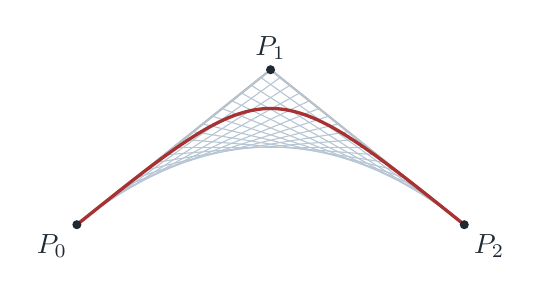
\begin{tikzpicture}[scale=0.82]
    \coordinate (P0) at (0,0);
    \coordinate (P1) at (3,2.4);
    \coordinate (P2) at (6,0);

    \draw[ynInk!35, thick] (P0)--(P1)--(P2);
    \foreach \i in {0,...,20} {
      \pgfmathsetmacro{\t}{\i/20}
      \coordinate (Q0) at ($(P0)!\t!(P1)$);
      \coordinate (Q1) at ($(P1)!\t!(P2)$);
      \draw[ynBlue!32] (Q0)--(Q1);
    }
    \draw[very thick, ynRed] (P0) .. controls (P1) .. (P2);
    \fill[ynInk] (P0) circle (2pt) node[below left] {\(P_0\)};
    \fill[ynInk] (P1) circle (2pt) node[above] {\(P_1\)};
    \fill[ynInk] (P2) circle (2pt) node[below right] {\(P_2\)};
  \end{tikzpicture}
  \caption{A smooth curve can appear as the envelope of many straight connector lines.}
  \label{fig:string-art-teaser}
\end{figure}

\begin{intuitionbox}
An envelope is a curve hidden inside a family. Each family member is simple, but the family as a whole has an edge, a ridge, or a curve of tangency. The visible curve is not one of the family members; it is produced by how nearby family members fit together.
\end{intuitionbox}

\section{Families of Curves}

An implicit plane curve can be described as the set of points satisfying an equation
\begin{align}
  F(x,y)=0.
\end{align}
For example, \(x+y=0\) is a line and \(y-x^2=0\) is a parabola.

To describe many related curves at once, introduce a parameter \(t\).

\begin{definitionbox}[title=One-parameter family of curves]
A \emph{one-parameter family of curves} is a collection
\begin{align}
  C_t=\set{(x,y)\in\R^2:F(x,y,t)=0},
\end{align}
where fixing \(t\) gives one curve from the family.
\end{definitionbox}

For instance,
\begin{align}
  F(x,y,t)=x+y+t
\end{align}
describes the family of parallel lines \(x+y+t=0\). Changing \(t\) shifts the line without rotating it.

Another family is
\begin{align}
  F(x,y,t)=y-tx-t^2.
\end{align}
Fixing \(t\) gives the line \(y=tx+t^2\). Here the slope changes with \(t\), and the lines form a visible curved boundary.

\begin{definitionbox}[title=Envelope]
An \emph{envelope} of a family \(C_t\) is a curve that is tangent to members of the family. Equivalently, in regular cases, it is the limiting locus of intersections of neighboring curves \(C_t\) and \(C_{t+h}\) as \(h\to 0\).
\end{definitionbox}

This second description is the one that leads directly to a calculation.

\section{The Envelope Conditions}

Assume \(F\) is differentiable in the parameter \(t\). A point on the curve \(C_t\) satisfies
\begin{align}
  F(x,y,t)=0.
\end{align}
If the same point is also on a nearby curve \(C_{t+h}\), then
\begin{align}
  F(x,y,t+h)=0.
\end{align}
Subtract the two equations:
\begin{align}
  F(x,y,t+h)-F(x,y,t)=0.
\end{align}
For \(h\neq 0\), divide by \(h\):
\begin{align}
  \frac{F(x,y,t+h)-F(x,y,t)}{h}=0.
\end{align}
Now let \(h\to 0\), holding the coordinates \((x,y)\) fixed while only the family parameter changes. The left side becomes the partial derivative of \(F\) with respect to \(t\):
\begin{align}
  \lim_{h\to0}
  \frac{F(x,y,t+h)-F(x,y,t)}{h}
  =
  \frac{\partial F}{\partial t}(x,y,t).
\end{align}
Thus a limiting intersection point must satisfy
\begin{align}
  F_t(x,y,t)=0.
\end{align}
It must also lie on the original curve \(C_t\). This gives the standard envelope conditions.

\begin{resultbox}
For a smooth one-parameter family \(F(x,y,t)=0\), envelope candidates are found by solving
\begin{align}
  \boxed{F(x,y,t)=0,\qquad F_t(x,y,t)=0.}
  \label{eq:envelope-conditions}
\end{align}
\end{resultbox}

The word ``candidates'' matters. The system in \cref{eq:envelope-conditions} can include singular or irrelevant branches. After solving it, we still have to check the geometry.

\begin{warningbox}[title=Two common mistakes]
Do not use \(F_t=0\) by itself. The point must also lie on a member of the family, so \(F=0\) is part of the system. Also, \(F_t\) is a partial derivative: while differentiating with respect to \(t\), the coordinates \(x\) and \(y\) are held fixed.
\end{warningbox}

\section{A Warm-Up: A Parabola from Lines}

Consider the family of lines
\begin{align}
  y=tx+t^2.
\end{align}
In implicit form,
\begin{align}
  F(x,y,t)=y-tx-t^2.
\end{align}
The partial derivative with respect to \(t\) is
\begin{align}
  F_t(x,y,t)=-x-2t.
\end{align}
The envelope conditions are therefore
\begin{align}
  y-tx-t^2&=0,\\
  -x-2t&=0.
\end{align}
The second equation gives
\begin{align}
  t=-\frac{x}{2}.
\end{align}
Substituting this into the line equation gives
\begin{align}
  y
    &=tx+t^2\\
    &=\paren{-\frac{x}{2}}x+\paren{-\frac{x}{2}}^2\\
    &=-\frac{x^2}{2}+\frac{x^2}{4}\\
    &=-\frac{x^2}{4}.
\end{align}

\begin{resultbox}
The envelope of the line family \(y=tx+t^2\) is the parabola
\begin{align}
  \boxed{y=-\frac{x^2}{4}.}
  \label{eq:parabola-envelope}
\end{align}
\end{resultbox}

This result is easy to check. The line with parameter \(t\) touches the parabola at \(x=-2t\). The derivative of the parabola is
\begin{align}
  \frac{\dd}{\dd x}\paren{-\frac{x^2}{4}}=-\frac{x}{2},
\end{align}
so at \(x=-2t\) the slope is \(t\), exactly the slope of the line \(y=tx+t^2\).

\begin{figure}[htbp]
  \centering
  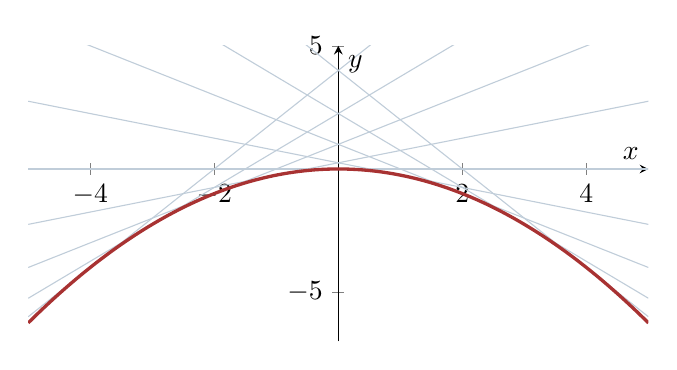
\begin{tikzpicture}
    \begin{axis}[
      width=0.78\linewidth,
      height=0.44\linewidth,
      axis lines=middle,
      xmin=-5,xmax=5,
      ymin=-7,ymax=5,
      xlabel={\(x\)},
      ylabel={\(y\)},
      samples=120,
      clip=true
    ]
      \foreach \m in {-2,-1.5,-1,-0.5,0,0.5,1,1.5,2} {
        \addplot[ynBlue!28, domain=-5:5, samples=2] {\m*x+\m*\m};
      }
      \addplot[very thick, ynRed, domain=-5:5] {-x^2/4};
    \end{axis}
  \end{tikzpicture}
  \caption{The line family \(y=tx+t^2\) is tangent to the envelope \(y=-x^2/4\).}
  \label{fig:line-parabola-envelope}
\end{figure}

\section{String Art and Quadratic Bezier Curves}

The straight-line construction from \cref{fig:string-art-teaser} has a precise formula. Let \(P_0,P_1,P_2\in\R^2\) be three control points. For \(0\leq t\leq 1\), define points moving along the two sides of the control polygon:
\begin{align}
  Q_0(t)&=(1-t)P_0+tP_1,\\
  Q_1(t)&=(1-t)P_1+tP_2.
\end{align}
For each \(t\), draw the line through \(Q_0(t)\) and \(Q_1(t)\). We will show that the envelope of these connector lines is the quadratic Bezier curve
\begin{align}
  B(t)=(1-t)^2P_0+2(1-t)tP_1+t^2P_2.
  \label{eq:quadratic-bezier}
\end{align}

To keep the derivation compact, use vector notation. Write a point in the plane as \(r=(x,y)\), and define
\begin{align}
  D(t)=Q_1(t)-Q_0(t).
\end{align}
The line through \(Q_0(t)\) and \(Q_1(t)\) consists of all points \(r\) for which \(r-Q_0(t)\) is parallel to \(D(t)\). In two dimensions, parallel vectors have determinant zero, so the line family is
\begin{align}
  F(r,t)=\det\paren{r-Q_0(t),D(t)}=0.
  \label{eq:bezier-line-family}
\end{align}

Differentiate \cref{eq:bezier-line-family} with respect to \(t\), holding \(r\) fixed:
\begin{align}
  F_t(r,t)
    &=
    \det\paren{-Q_0'(t),D(t)}
    +
    \det\paren{r-Q_0(t),D'(t)}\\
    &=
    -\det\paren{Q_0'(t),D(t)}
    +
    \det\paren{r-Q_0(t),D'(t)}.
\end{align}
Any point on the line can be written as
\begin{align}
  r=Q_0(t)+\lambda D(t),
\end{align}
for some line coordinate \(\lambda\). Substituting this into \(F_t=0\) gives
\begin{align}
  0
    &=
    -\det\paren{Q_0'(t),D(t)}
    +
    \lambda\det\paren{D(t),D'(t)}.
  \label{eq:lambda-envelope-condition}
\end{align}

Now set
\begin{align}
  A=P_1-P_0,\qquad C=P_2-2P_1+P_0.
\end{align}
Then
\begin{align}
  Q_0'(t)&=A,\\
  D(t)&=A+tC,\\
  D'(t)&=C.
\end{align}
Therefore
\begin{align}
  \det\paren{Q_0'(t),D(t)}
    &=\det\paren{A,A+tC}
      =t\det\paren{A,C},\\
  \det\paren{D(t),D'(t)}
    &=\det\paren{A+tC,C}
      =\det\paren{A,C}.
\end{align}
If the control points are not collinear, \(\det(A,C)\neq 0\). Equation \cref{eq:lambda-envelope-condition} becomes
\begin{align}
  0=-t\det(A,C)+\lambda\det(A,C),
\end{align}
so
\begin{align}
  \lambda=t.
\end{align}
The envelope point on the connector line is thus
\begin{align}
  r
    &=Q_0(t)+tD(t)\\
    &=(1-t)Q_0(t)+tQ_1(t)\\
    &=(1-t)\bigl((1-t)P_0+tP_1\bigr)
      +t\bigl((1-t)P_1+tP_2\bigr)\\
    &=(1-t)^2P_0+2(1-t)tP_1+t^2P_2.
\end{align}

\begin{resultbox}
The envelope of the connector lines is the quadratic Bezier curve
\begin{align}
  \boxed{
  B(t)=(1-t)^2P_0+2(1-t)tP_1+t^2P_2,
  \qquad 0\leq t\leq 1.
  }
\end{align}
\end{resultbox}

Two endpoint checks make the geometry clearer:
\begin{align}
  B(0)&=P_0,&
  B(1)&=P_2,\\
  B'(0)&=2(P_1-P_0),&
  B'(1)&=2(P_2-P_1).
\end{align}
So the first and last control segments determine the incoming and outgoing tangent directions of the curve.

\begin{checkpointbox}
The finite string-art picture is an approximation: it uses only finitely many connector lines. The exact envelope belongs to the continuous family, where every \(t\in[0,1]\) contributes one line.
\end{checkpointbox}

\section{Caustics Are Envelopes of Rays}

We can now return to the bright curve in the mug. In geometric optics, light is modeled by rays. A smooth reflecting wall turns incoming rays into outgoing rays according to the law of reflection. Each reflected ray is a line or half-line, and the bright visible curve is the envelope of that ray family.

\begin{definitionbox}[title=Caustic]
A \emph{caustic} is a curve or surface where reflected or refracted rays concentrate. A caustic produced by reflection is also called a \emph{catacaustic}.
\end{definitionbox}

The key physical point is simple: rays do not have to collide with one another. The bright curve appears because nearby reflected rays pass close together, increasing the local ray density.

\section{An Ideal Circular-Cup Model}

The real mug is three-dimensional, slightly imperfect, and illuminated by a finite light source. To get a clean calculation, we use an ideal two-dimensional model.

\begin{itemize}
  \item The cup wall is a circle of radius \(R\).
  \item Incoming rays are parallel and travel in direction \(d=(1,0)\).
  \item Reflection is specular: the normal component of the incoming direction reverses.
  \item We first set \(R=1\), then scale the final result by \(R\).
\end{itemize}

Parametrize the circular wall by
\begin{align}
  P(\theta)=(\cos\theta,\sin\theta),
  \qquad
  n(\theta)=(\cos\theta,\sin\theta),
\end{align}
where \(n(\theta)\) is the outward unit normal. Reflection across the tangent line is computed by subtracting twice the normal component:
\begin{align}
  v(\theta)=d-2\paren{d\cdot n(\theta)}n(\theta).
\end{align}
Since \(d=(1,0)\), we have \(d\cdot n(\theta)=\cos\theta\), and hence
\begin{align}
  v(\theta)
    &=(1,0)-2\cos\theta(\cos\theta,\sin\theta)\\
    &=(1-2\cos^2\theta,-2\sin\theta\cos\theta)\\
    &=(-\cos2\theta,-\sin2\theta).
  \label{eq:reflected-direction}
\end{align}
The reflected ray line at angle \(\theta\) is
\begin{align}
  \ell_\theta(s)=P(\theta)+s\,v(\theta),
  \qquad s\in\R.
  \label{eq:ray-parametric}
\end{align}
The physical reflected ray is only one half of this line, but the full line is convenient for finding the envelope.

\begin{figure}[htbp]
  \centering
  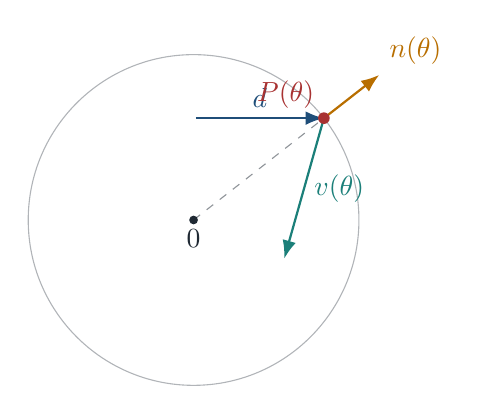
\begin{tikzpicture}[scale=1.05, >=Latex]
    \coordinate (O) at (0,0);
    \coordinate (P) at (38:2);
    \draw[ynInk!35] (O) circle (2);
    \draw[ynInk!50, dashed] (O)--(P);
    \draw[->, thick, ynBlue] ($(P)+(-1.55,0)$)--(P) node[midway, above] {\(d\)};
    \draw[->, thick, ynTeal] (P)--($(P)+(-0.48,-1.7)$) node[midway, right] {\(v(\theta)\)};
    \draw[->, thick, ynAmber] (P)--($(P)+(38:0.85)$) node[above right] {\(n(\theta)\)};
    \fill[ynInk] (O) circle (1.5pt) node[below] {\(0\)};
    \fill[ynRed] (P) circle (2pt) node[above left] {\(P(\theta)\)};
  \end{tikzpicture}
  \caption{In the ideal model, the reflected direction is obtained by reversing the normal component of the incoming direction.}
  \label{fig:reflection-geometry}
\end{figure}

\subsection{Finding the ray envelope}

For a line family in vector form
\begin{align}
  r=P(\theta)+s\,v(\theta),
\end{align}
one efficient envelope formula is
\begin{align}
  s(\theta)
  =
  \frac{\det\paren{P'(\theta),v(\theta)}}
       {\det\paren{v(\theta),v'(\theta)}}.
  \label{eq:line-family-envelope-s}
\end{align}
Here is the derivation. The line through \(P(\theta)\) in direction \(v(\theta)\) has implicit equation
\begin{align}
  F(r,\theta)=\det\paren{r-P(\theta),v(\theta)}=0.
\end{align}
Differentiate with respect to \(\theta\), holding \(r\) fixed:
\begin{align}
  F_\theta
    &=
    -\det\paren{P'(\theta),v(\theta)}
    +
    \det\paren{r-P(\theta),v'(\theta)}.
\end{align}
On the line, \(r-P(\theta)=s\,v(\theta)\). Therefore the envelope condition \(F_\theta=0\) gives
\begin{align}
  0
    &=
    -\det\paren{P'(\theta),v(\theta)}
    +
    s\det\paren{v(\theta),v'(\theta)}.
\end{align}
Solving for \(s\) gives \cref{eq:line-family-envelope-s}, provided the denominator is nonzero.

Now compute the terms for our circular model:
\begin{align}
  P'(\theta)&=(-\sin\theta,\cos\theta),\\
  v(\theta)&=(-\cos2\theta,-\sin2\theta),\\
  v'(\theta)&=(2\sin2\theta,-2\cos2\theta).
\end{align}
The determinants are
\begin{align}
  \det\paren{P'(\theta),v(\theta)}
    &=
    (-\sin\theta)(-\sin2\theta)
    -(\cos\theta)(-\cos2\theta)\\
    &=
    \sin\theta\sin2\theta+\cos\theta\cos2\theta\\
    &=
    \cos\theta,
\end{align}
and
\begin{align}
  \det\paren{v(\theta),v'(\theta)}
    &=
    (-\cos2\theta)(-2\cos2\theta)
    -(-\sin2\theta)(2\sin2\theta)\\
    &=2.
\end{align}
Thus
\begin{align}
  s(\theta)=\frac{\cos\theta}{2}.
\end{align}
Substitute this into the ray equation:
\begin{align}
  c(\theta)
    &=P(\theta)+\frac{\cos\theta}{2}v(\theta)\\
    &=(\cos\theta,\sin\theta)
      +\frac{\cos\theta}{2}(-\cos2\theta,-\sin2\theta).
\end{align}
Componentwise,
\begin{align}
  x(\theta)
    &=\cos\theta-\frac{\cos\theta\cos2\theta}{2},\\
  y(\theta)
    &=\sin\theta-\frac{\cos\theta\sin2\theta}{2}.
\end{align}
Using
\begin{align}
  \cos\theta\cos2\theta
    &=\frac{\cos3\theta+\cos\theta}{2},\\
  \cos\theta\sin2\theta
    &=\frac{\sin3\theta+\sin\theta}{2},
\end{align}
we obtain
\begin{align}
  x(\theta)
    &=
    \cos\theta-\frac{\cos3\theta+\cos\theta}{4}
     =
    \frac{3\cos\theta-\cos3\theta}{4},\\
  y(\theta)
    &=
    \sin\theta-\frac{\sin3\theta+\sin\theta}{4}
     =
    \frac{3\sin\theta-\sin3\theta}{4}.
\end{align}
Scaling back to a circle of radius \(R\) gives the ideal caustic:
\begin{align}
  \boxed{
  c_R(\theta)=
  R\paren{
  \frac{3\cos\theta-\cos3\theta}{4},
  \frac{3\sin\theta-\sin3\theta}{4}
  }.
  }
  \label{eq:nephroid-caustic}
\end{align}

\begin{warningbox}[title=Modeling caveat]
\Cref{eq:nephroid-caustic} is the caustic for an ideal circular cross-section with parallel incoming rays under the stated orientation. A real mug can show only part of this curve, and the visible shape can be rotated, clipped, blurred, or distorted by the light source, cup geometry, and three-dimensional projection.
\end{warningbox}

\begin{figure}[htbp]
  \centering
  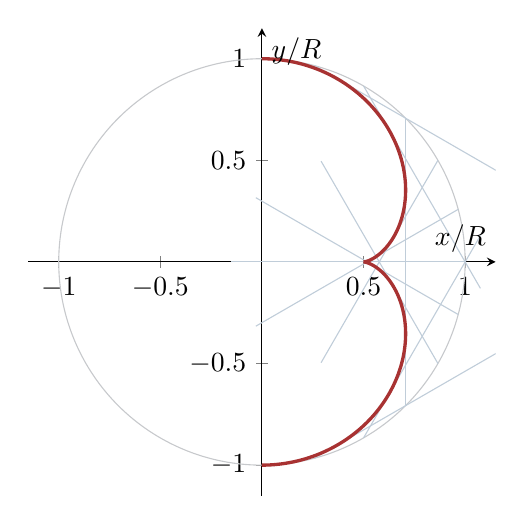
\begin{tikzpicture}
    \begin{axis}[
      width=0.78\linewidth,
      height=0.62\linewidth,
      axis equal image,
      xmin=-1.15,xmax=1.15,
      ymin=-1.15,ymax=1.15,
      axis lines=middle,
      xlabel={\(x/R\)},
      ylabel={\(y/R\)},
      xtick={-1,-0.5,0,0.5,1},
      ytick={-1,-0.5,0,0.5,1},
      samples=160,
      clip=true
    ]
      \addplot[ynInk!25, domain=0:360, samples=260]
        ({cos(x)},{sin(x)});
      \foreach \a in {-75,-60,-45,-30,-15,0,15,30,45,60,75} {
        \addplot[ynBlue!28, domain=0:1.15, samples=2]
          ({cos(\a)-x*cos(2*\a)},{sin(\a)-x*sin(2*\a)});
      }
      \addplot[very thick, ynRed, domain=-90:90, samples=260]
        ({(3*cos(x)-cos(3*x))/4},{(3*sin(x)-sin(3*x))/4});
    \end{axis}
  \end{tikzpicture}
  \caption{In the ideal circular model, the caustic is the envelope of reflected ray lines. The plotted arc corresponds to one visible family of reflected rays.}
  \label{fig:cup-caustic}
\end{figure}

\section{What to Remember}

The same mechanism explains all three examples in the note:
\begin{enumerate}
  \item Model a family of curves \(F(x,y,t)=0\).
  \item Add the derivative condition \(F_t(x,y,t)=0\).
  \item Solve the two equations together.
  \item Check that the result is geometrically the envelope you intended.
\end{enumerate}

\begin{checkpointbox}
Quick checks:
\begin{itemize}
  \item Parallel lines \(F(x,y,t)=x-t\) have \(F_t=-1\), so the envelope system has no solution.
  \item For \(y=tx+t^2\), the line with parameter \(t\) is tangent to \(y=-x^2/4\) at \(x=-2t\).
  \item For the string-art construction, \(B(0)=P_0\), \(B(1)=P_2\), and the endpoint tangents point along \(P_0P_1\) and \(P_1P_2\).
  \item For the caustic, the formula scales linearly with the cup radius \(R\), so the dimensions are consistent.
\end{itemize}
\end{checkpointbox}

\section{Exercises}

\begin{enumerate}
  \item Find the envelope of the family \(F(x,y,t)=y-tx+t^2=0\). Compare it with \cref{eq:parabola-envelope}.
  \item Let \(F(x,y,t)=(x-t)^2+y^2-1\). Solve \(F=0\) and \(F_t=0\). Interpret the two envelope branches geometrically.
  \item For the quadratic Bezier curve \(B(t)\), verify directly that
  \[
    B'(t)=2\bigl(Q_1(t)-Q_0(t)\bigr).
  \]
  Explain why this confirms that the connector line is tangent to the curve.
  \item In the cup model, check that the reflected direction \(v(\theta)=(-\cos2\theta,-\sin2\theta)\) has unit length for all \(\theta\).
  \item Evaluate \cref{eq:nephroid-caustic} at \(\theta=0,\pi/2,\pi\). Sketch these points on the unit circle and explain what they say about the caustic.
\end{enumerate}

\section{Conclusion}

An envelope is a way for a curve to be present without being drawn directly. It is encoded by a whole family of nearby curves: tangent lines, connector lines, or reflected light rays. The calculus condition \(F_t=0\) captures the limiting-intersection intuition, while the original condition \(F=0\) keeps the point on the family member. Together they turn a visual phenomenon into a method:
\begin{align}
  \text{family} + \text{neighboring-intersection limit}
  \quad\longrightarrow\quad
  \text{envelope}.
\end{align}
That method is why a pattern of straight lines can hide a Bezier curve, and why the bottom of a mug can reveal a bright mathematical curve made by light.

\end{document}
